%----------------------------------------------------------------------------------------
%	SYGNATURE PAGE
%----------------------------------------------------------------------------------------
\newpage
\thispagestyle{plain}
%\addcontentsline{toc}{chapter}{\protect\numberline{}Sobre o autor}
\phantomsection
\addcontentsline{toc}{chapter}{\protect\numberline{}Sobre o autor}

%\addvspace{12pt}\Huge\bfseries\textit{Sobre o autor}
\begin{figure}[H]
	\flushright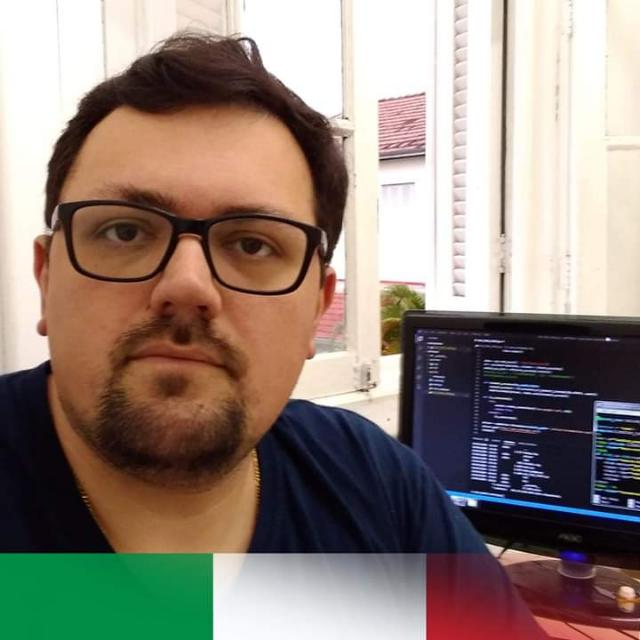
\includegraphics[width=.2\linewidth]{Pictures/eu01.jpg}
	\label{fig:eu}
\end{figure}
\newcommand*{\tituloautor}{\addvspace{12pt}\Huge\fontfamily{yes}\selectfont}
\newcommand*{\descricaoautor}{\fontfamily{yes}\selectfont}
{\tituloautor\textbf{Sobre o Autor}}
\\
\\
{\descricaoautor{O Prof. Dr. Edson Fernando \textbf{Fumachi} nasceu em Itatiba-SP em 18 de Maio de 1983. Estudou em escolas públicas até o ensino médio. Ingressou no ano 2001 no Curso de Licenciatura em Matemática na Universidade São Francisco, obtendo seu título em 2003. Em 2004 começou a trabalhar no ensino superior da mesma faculdade na qual se graduou. No ano de 2005 assumiu a posição de professor PEB-II do Governo do Estado de São Paulo na disciplina de Matemática. Exonerou do cargo em 2007 para dar sequência no ensino superior. Trabalhou como professor do ensino médio público e privado; no ensino médio privado atuou como professor de Matemática e Física. Em 2007 começou seus estudos como aluno de matéria isolada no Instituto Nacional de Pesquisas Espaciais - INPE, localizado em São José dos Campos-SP. Em 2009 entrou no mesmo instituto como aluno regular do Curso de Mestrado em Engenharia e Tecnologia Espaciais área de concentração em Ciência e Tecnologia dos Materiais e Sensores. Em 2011 defendeu sua Dissertação intitulada \textit{Simulação do fluxo reacional de um reator de filamento quente através da simulação direta de Monte Carlo}. Consecutivamente, em 2011, ingressou no Curso de Doutorado na mesma área do mesmo instituto. Em 2017 defendeu seu Doutorado intitulado \textit{Desenvolvimento de um tubo de queda livre para o modelamento e otimização do processo de solidificação de ligas eutéticas de bismuto-estanho em ambiente de microgravidade}. Tem experiência no meio empresarial através de consultorias realizadas na área de telecomunicações e desenvolvimento de algoritmos para otimização de processos e redução de custos. Tem amplo conhecimento em programação de computadores nas linguagens ForTran77, C e Python. Desenvolve materiais didáticos (como este!) em diversos formatos e linguagens (\LaTeX). Desenvolve conteúdos educacionais e os disponibiliza em plataformas digitais, Youtube e Facebook, sob o pseudônimo Doutor Exatas. }}






